\section{Biological background}
\subsection{Amino-acid residues}
\textbf{Amino acids} are the building blocks of proteins and play a fundamental role in various biological processes. These small organic molecules are essential for life, and their unique properties allow them to form complex and diverse structures within the body. 
All amino acids follow the same underlying pattern and consist of a central carbon atom (C), an \textit{amino} group ($\text{NH}_3$), a \textit{carboxyl} group (COOH), and a variable side-chain, as we can see in Figure \ref{fig:amino-acid}.
Chains of amino acids are formed through a chemical reaction that creates a \textit{peptide bond}, as shown in Figure \ref{fig:residue}. The portions left of the original amino acids are called \textit{residues}. Note that there are 20 naturally occuring amino acids.
\begin{figure}
    \centering
    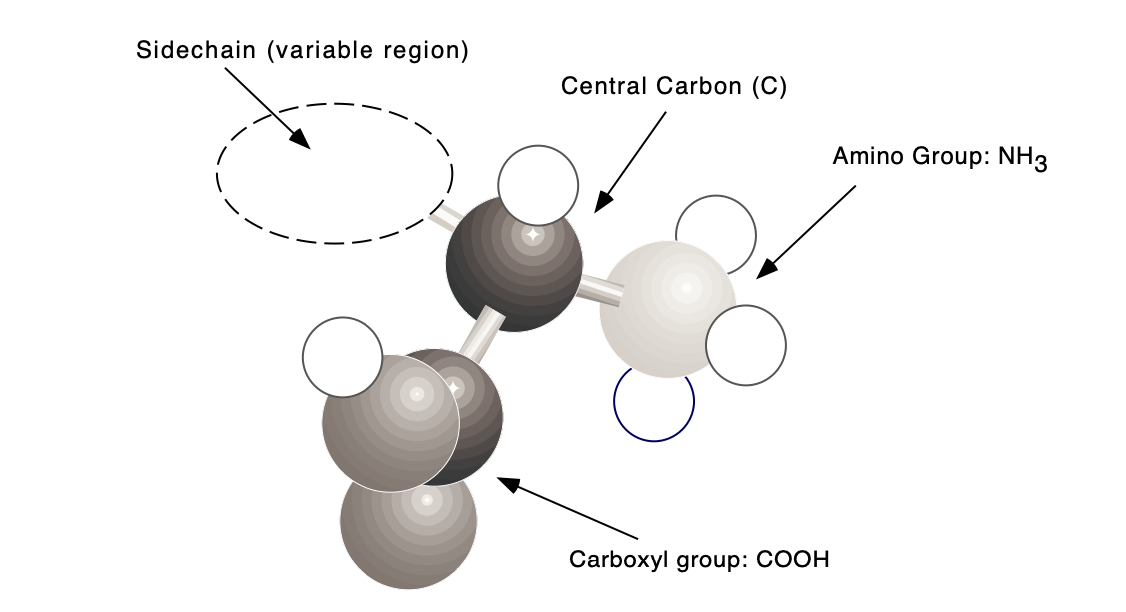
\includegraphics[scale=0.5]{figures/amino-acid.png}
    \caption{The basic chemical structure of an amino acid. Carbon atoms are black, Oxygen is dark grey, Nitrogen light grey, and hydrogen white. Image taken from \cite{hunter1993molecular}.}
    \label{fig:amino-acid}
\end{figure}

\begin{figure}
    \centering
    \begin{tikzpicture}
    \node (acidone) {\chemfig[atom sep=2em]{N(-[3]H)(-[5]H)-C(-[2]H)(-[6]R_1)-C(-[1]{\color{blue}OH})(=[7]O)}};
    \node[right of=acidone, xshift=3cm] (acidtwo) {\chemfig[atom sep=2em]{N(-[3]H)(-[5]{\color{blue}H})-C(-[2]H)(-[6]R_2)-C(-[1]OH)(=[7]O)}};
    \draw[->,thick] ($(acidone.east)!0.5!(acidtwo.west)$) ++(0, -1.2cm) -- ++(0,-0.8cm) node[right] {};
    \node[below of=acidone, xshift=2cm, yshift=-2.4cm] (residue) 
        {\chemfig[atom sep=2em]{N(-[3]H)(-[5]H)-C(-[2]H)(-[6]R_1)-C(=[7]O)-[1,,,,blue]N(-[3]H)-C(-[2]H)(-[6]R_2)-C(=[7]O)(-[1]OH)}};
    
    \node[below of=residue, yshift=-0.7cm, xshift=-1.5cm] (res1) {\textit{residue 1}};
    \node[below of=residue, yshift=-0.7cm, xshift=1.5cm] (res1) {\textit{residue 2}};
    \end{tikzpicture}
    \caption{Two amino-acids are chained together through a peptide bond. The chemical reaction releases a water molecule ($\text{H}_2\text{O}$) in the process.}
    \label{fig:residue}
\end{figure}

\subsection{Proteins}
Multiple amino-acids chained together through peptide bonds form a \textit{polypeptide chain}.
These chains fold into shapes, forming \textbf{proteins}. 
Proteins are one of the most important macromolecules found in living organisms and they are involved in a vast array of biological processes. 
Proteins play a variety of roles in the body, including catalysing chemical reactions, transporting molecules, providing structural support, and regulating gene expression. 
The diversity of protein structures and functions is vast, with some proteins consisting of just a few amino acids, while others contain thousands. 
The unique sequence of amino acids in each protein determines its three-dimensional structure and, more importantly, its \textit{specific function}. 
Understanding the structure and function of proteins is essential for advancing our knowledge of cellular processes and for developing treatments for a range of diseases caused by protein dysfunction.

\paragraph{Biological assemblies.}
Proteins can further fold together into protein complexes, also known as \textit{biological assemblies}.
These assemblies can be composed of multiple copies of the same protein (\textit{homomeric assemblies}) or different protein molecules (\textit{heteromeric assemblies}).
Heteromeric assemblies can also contain other types of molecules, such as  nucleic acids or lipids. Figure \ref{assembly} shows an example of a homomeric assembly.
\begin{figure}
    \centering
    \subfigure[The 2UXY molecule. It is formed of a single chain of amino-acid residues.]{
        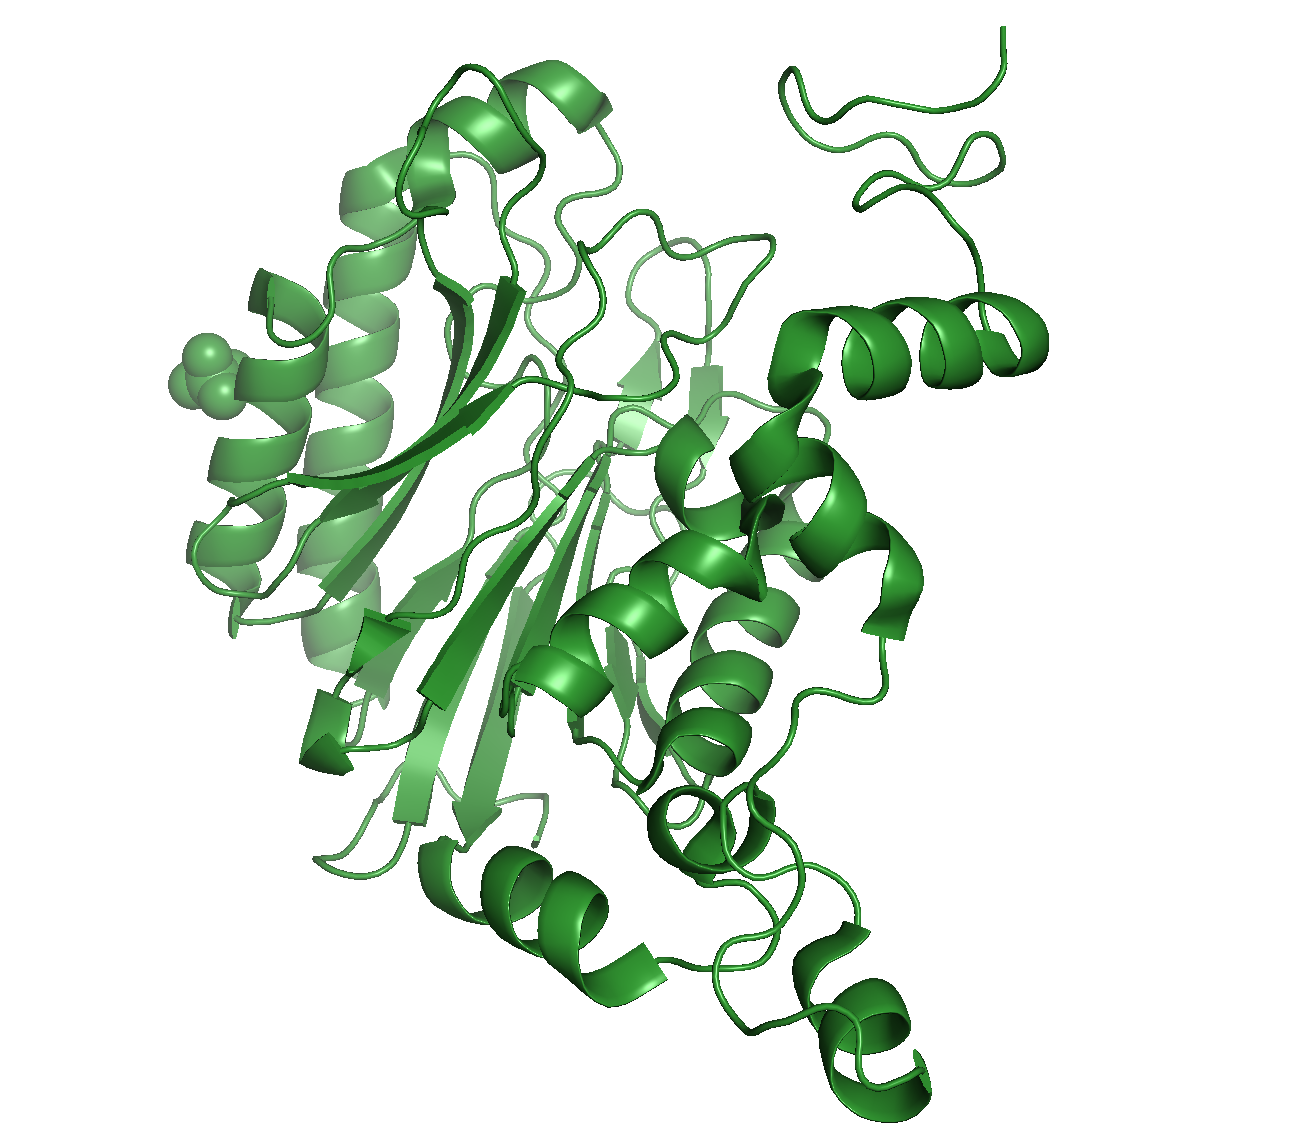
\includegraphics[scale=0.3]{figures/2uxy.png}
        \label{homomer}
    }
    \hspace{0.3in}
    \subfigure[The \textit{aliphatic amidase} assembly, formed of 6 copies of the 2UXY chain.]{
        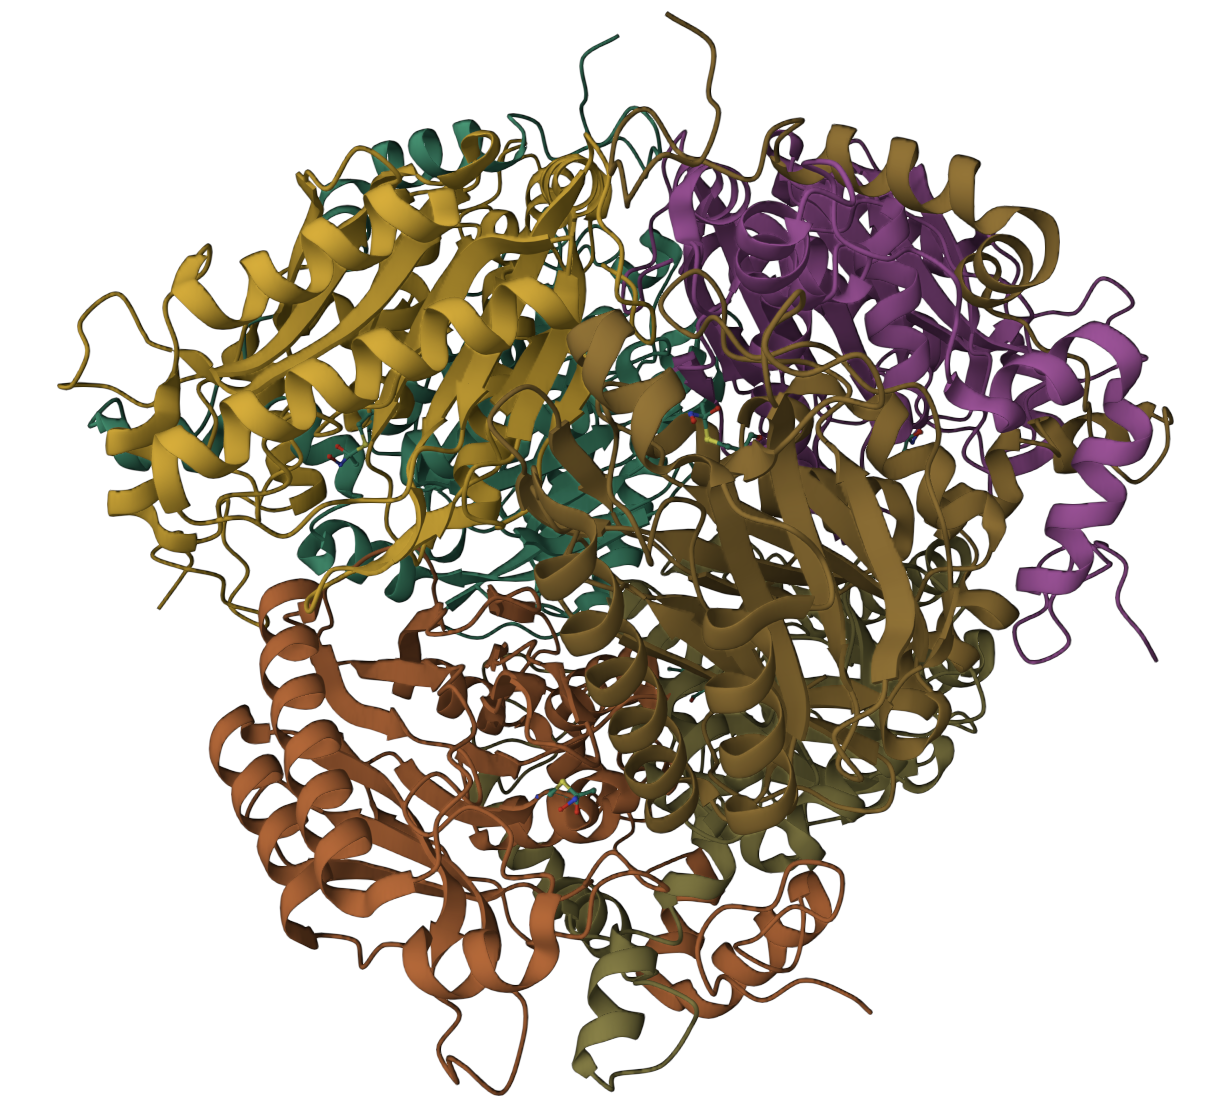
\includegraphics[scale=0.3]{figures/2uxy_assembly.png}
    }
    \caption{Example of (a) one homomer and  (b) the homomeric assembly it forms.}
    \label{assembly}
\end{figure}

\paragraph{Protein engineering.}
Protein engineering is the task of designing new proteins that have specific functions.
One way in which we can perform protein engineering is by swapping out amino-acid residues within a chain with potentially more efficient ones.
This approach involves particularly challenging design choices when dealing with biological assemblies: while we can isolate a monomer in the lab to study its properties, in real life this monomer will not function by itself, but rather bind to other proteins to execute a certain function.
Hence, when performing a mutation on a single-chain protein that is known to be part of a biological assembly, we must propagate this mutation to all other instances of this protein within the assembly.

\paragraph{Protein representations.}
The structure of a protein can be classified into the primary, secondary, and tertiary structure:
\begin{enumerate}
\item The primary structure of a protein refers to the linear sequence of amino acids in the protein chain. 
It is determined by the specific order of amino acids linked together by peptide bonds, forming the polypeptide chain. The primary structure of a protein is the most basic level of protein structure and dictates the overall chemical properties and function of the protein.
\item Next, the secondary structure of a protein refers to the local folding patterns or motifs that arise from interactions between nearby amino acids in the polypeptide chain. 
The most common types of secondary structures are alpha helices and beta sheets.
\item Lastly, the tertiary structure of a protein refers to the overall three-dimensional arrangement of the polypeptide chain, including the long-range interactions and folding patterns that determine the protein's geometric shape. 
The tertiary structure is stabilised by various interactions, including hydrogen bonding, disulfide bonds, van der Waals forces, hydrophobic interactions, and electrostatic interactions. The tertiary structure is critical for the protein's function and determines its specific shape, stability, and activity.
\end{enumerate}

The \textbf{Protein Data Bank} (PDB) is a publicly accessible online repository that stores and provides access to three-dimensional structural data of biological macromolecules, primarily proteins and nucleic acids. 
The PDB is a global resource that serves as a central repository for experimentally determined structures of biomolecules obtained through techniques such as X-ray crystallography, NMR spectroscopy, and cryo-electron microscopy.
Within the PDB, researchers can download \texttt{.pdb} files, that typically represent the three-dimensional structure of a protein at the atomic level, which includes the primary, secondary, and tertiary structures of the protein. 
PDB files contain information about the 3D coordinates of individual atoms in the protein, as well as information about the type of amino acids, secondary structure elements, and other structural features present in the protein.


\subsection{Residue identity prediction}
Residue identity prediction (RES) is a computational task in bioinformatics that involves predicting the amino acid residue at a particular position within a protein sequence. 
The accurate prediction of residue identity is an important problem in bioinformatics because it can provide insights into protein function, structure, and evolution. 
Knowing the identity of residues within a protein sequence can help to identify important functional sites and motifs, which can provide clues about the protein's function and interactions with other molecules. 

Residue identity prediction is also important for \textit{protein engineering}, as it can help researchers design proteins with specific functions.
Machine learning approaches to RES have already been used to engineer plastic decomposing enzymes for higher thermal stability \cite{Lu2022}.

\paragraph{The ATOM3D dataset.} One important benchmark dataset for RES is ATOM3D \cite{atom-3d}.
The ATOM3D collection is a compilation of datasets that contain the 3D structure of biomolecules, including nucleic acids, small molecules, and proteins. 
These datasets have been tailored to function as a benchmark for machine learning techniques that train on the 3D molecular structure of molecules in order to solve tasks such as molecular function prediction, ligand binding affinity, or protein-protein interactions.

\section{Machine learning background}
First proposed by \citet{rosenblatt1958}, neural networks are a type of machine learning model that is inspired by the structure and function of the human brain. 
They are used for various tasks, such as image and speech recognition, natural language processing, and biomolecular prediction among others.

At a high level, neural networks consist of interconnected nodes or neurons organised into layers. Each neuron receives input data, applies a mathematical operation to it, and produces an output. These operations are typically weighted sums followed by activation functions that introduce non-linearity into the model. 
The outputs from one layer of neurons serve as inputs to the next layer, forming a hierarchical structure. The resulting predictions made by the model are then scored using a \textit{loss function}.

The training process in neural networks involves two steps. First, the derivative of the loss function with respect to each weight is computed, using the \textit{backpropagation algorithm} \citep{backpropagation1}. This provides the gradient information needed for the next step. The second stage is the weight update, typically done using a gradient descent technique. 

\subsection{Graph Neural Networks}
{\color{blue}Maybe flesh this out later.}

\textbf{Graph neural networks} (GNNs) are a type of neural network that operate on graphs and are able to capture structural information in the data by leveraging the existent relationships between entities. 
All GNNs use some form of \textit{neural message passing}, where vector messages are exchanged between nodes and updated using a neural network \citep{gilmer2017neural}.

Formally, for a given graph $\mathcal{G} = (\mathcal{V}, \mathcal{E})$, at message passing iteration $k$, a hidden embedding $\textbf{h}_u^{(k)} \in \mathbb{R}^{F_k}$ corresponds to each node $u \in \mathcal{V}$. 
The framework first creates a \textit{message} $\mathbf{m}_{u,v}$ between a node $u$ and its neighbour $v$ by using a message function $\psi^{(k)}: \mathbb{R}^{F_k}\times\mathbb{R}^{F_k} \rightarrow \mathbb{R}^{F_{k}'}$:
\begin{equation}
    \mathbf{m}_{u, v} = \psi^{(k)}\Big(\textbf{h}_{u}^{(k)}, \textbf{h}_v^{(k)}\Big)
\end{equation}
These messages are then aggregated using operation $\oplus^{(k)}$; 
this operation is usually the sum or the average, but other versions exist as well. Note that in general function must be \textit{permutation invariant}, since the neighbours of a node $u$ do not have any intristic order.
Finally, the aggregated message is combined with the node's own embedding $\mathbf{h}_u^{(k)}$ using function $\phi^{(k)}:\mathbb{R}^{F_k} \times \mathbb{R}^{F_{k}'} \rightarrow \mathbb{R}^{F_{k+1}}$, also called the \textit{update} function, as seen in Equation \ref{message-passing}:
\begin{align}
    \textbf{h}_u^{(k+1)} &= \phi^{(k)}\Big(\textbf{h}_u^{(k)}, \oplus_{v\in \mathcal{N}(u)}^{(k)}\mathbf{m}_{u,v}\Big)
\label{message-passing}
\end{align}

A visual representation of the information flow can be seen in Figure \ref{message_passing_fig}.
\begin{figure}
    \centering
    \begin{tikzpicture}[scale=0.6]
        % Graph
        \node (x1) [circle, draw=black, fill=red!20] {$\mathbf{x}_1$};
        \node (x2) [circle, draw=black, thick, fill=blue!20, below of=x1, yshift=-2cm, xshift=-4cm] {$\mathbf{x}_2$};
        \node (x3) [circle, draw=black, fill=blue!20, below of=x1, yshift=-2cm, xshift=4cm] {$\mathbf{x}_3$};
        \node (x4) [circle, draw=black, fill=blue!20, below of=x1, yshift=-2.5cm, xshift=1cm] {$\mathbf{x}_4$};

        
        \draw (x1) -- (x2);
        \draw (x1) -- (x3);
        \draw (x1) -- (x4);

        % Messages
        \node (m12) [circle, fill=green!30, above=of x2.center, xshift=0.7cm, yshift=0.3cm] {$\mathbf{m}_{1,2}$};
        \node (m13) [circle, fill=green!30, above=of x3.center, xshift=-0.7cm, yshift=0.3cm] {$\mathbf{m}_{1,3}$};
        \node (m14) [circle, fill=green!30, above=of x4.center, xshift=-1.3cm] {$\mathbf{m}_{1,4}$};

        \draw [->, dashed, gray, line width=1pt] (x1) -- (m14);
        \draw [->, dashed, gray, line width=1pt] (x4) -- (m14);
        % \draw [->, line width=2.5pt] (up1) .. controls (-0.25, 0.6) .. (x1);
        \draw [->, dashed, gray, line width=1pt] (x2) -- (m12);
        \draw [->, dashed, gray, line width=1pt] (x1) -- (m12);

        \draw [->, dashed, gray, line width=1pt] (x3) -- (m13);
        \draw [->, dashed, gray, line width=1pt] (x1) -- (m13);

        \node (update1) [circle, fill=orange!20, above=of x1.center, yshift=1cm] {$\oplus$};
        % \draw [->, line width=1.5pt] (m12) .. controls (-3, 0.5) .. (update1);
        \path (m12) edge[->, line width=1.2pt, bend left=30] (update1);
        \path (m14) edge[->, line width=1.2pt, bend left=30] (update1);
        \path (m13) edge[->, line width=1.2pt, bend right=30] (update1);
        \path (x1) edge[->, dashed, gray, line width=1pt, bend right=45] (update1);

        \draw [->, double, double distance=1pt, line width=1pt] (update1) -- (x1);
        \draw (x2) -- (x4);

        % \draw [->, line width=2pt] (m13) -- (up1);
    \end{tikzpicture}
    \caption{Diagram of the information flow of Equation \ref{message-passing}. Node $\mathbf{x}_1$ has three neighbours coloured in blue. The messages between node $\mathbf{x}_1$ and each of its neighbours are aggregated using operator $\oplus$; the result is used to update the embeddings of $\mathbf{x}_1$. Note how in this diagram we are not interested in the edge between $\mathbf{x}_2$ and $\mathbf{x}_4$, since this is the update iteration for node 1.}
    \label{message_passing_fig}
\end{figure}
\subsection{Equivariant Graph Neural Networks}
Note how each message-passing iteration in a GNN must be permutation invariant, since changing the node ordering of a graph results in the same permutation applied to the node outputs of the layer. 
The overall GNN model is also permutation invariant, since graph-level property predictions should not be affected by the order we assign to nodes when processing them.

While permutation equivariance and invariance is sufficient when dealing with graphs that only represent relational information (e.g., social networks), in this project we are interested in graphs that do not only encode relationships, but also geometric information: the atoms of a protein have both 3D coordinates and features.
Hence, we are interested in developing message passing layers that obey \textbf{translation} and \textbf{rotation equivariance}. Briefly, this means that structural properties (such as volumes, distance, velocity, and relative positioning) are preserved across layers, as shown in Figure \ref{equivariance}. 
\begin{figure}
    \centering
    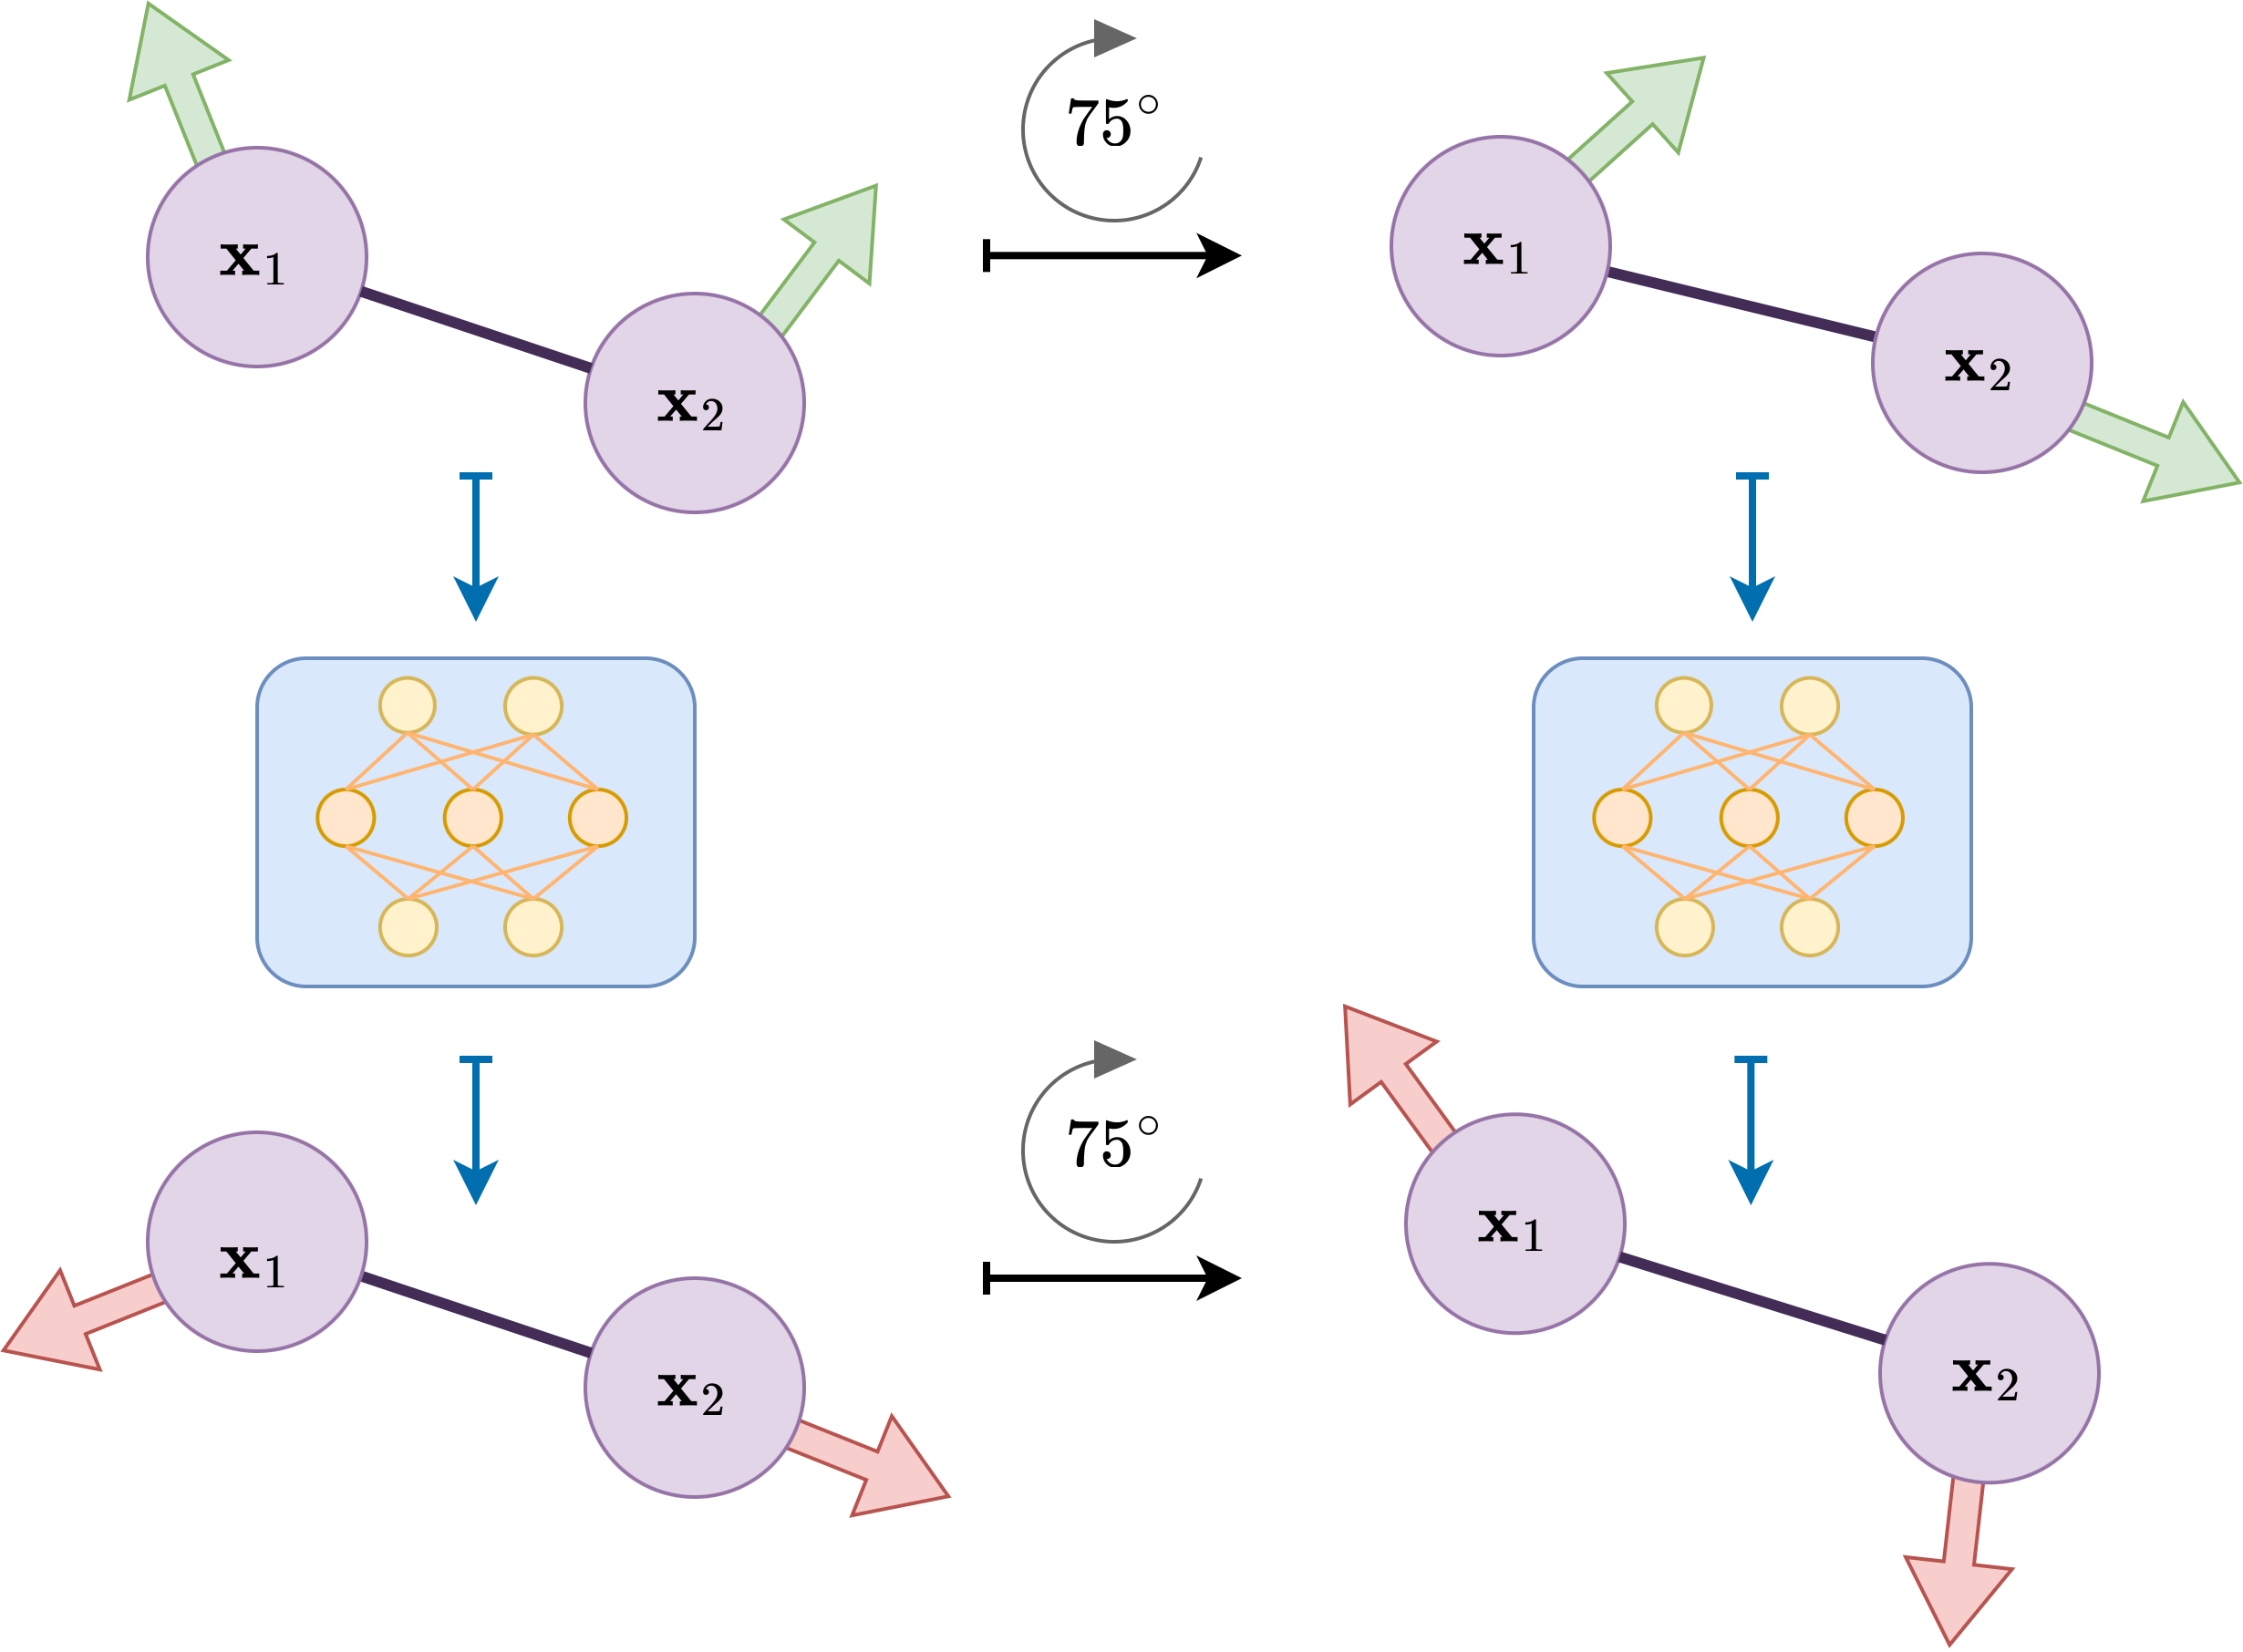
\includegraphics[scale=0.7]{figures/equivariance-2.png}
    \caption{Visual representation of rotation equivariance. If the input graph has nodes with 3D coordinates (represented by the green and red arrows) and is rotated by a certain degree, we expect that the output graph will be rotated in a predictible manner as well.}
    \label{equivariance}
\end{figure}

\subsection{Equivariance formalism}
Formally, for message-passing iteration $\ell$, given a $\mathbf{H}^{\ell}\in\mathbb{R}^{n \times d}$ matrix of node features for a given molecular graph, where $n$ is the number of nodes (i.e., atoms) and each row $\mathbf{h}^{\ell}_i$ is the $d-$dimensional feature of node $i$; a $\textbf{X}^{\ell}\in \mathbb{R}^{n \times 3}$ matrix of node coordinates for the molecular graph, where $\mathbf{x}^{\ell}_i$ is the 3D coordinate of node $i$; and the $\mathbf{A}\in\mathbb{R}^{n \times n}$ adjancency matrix, 
we have a GNN layer $\mathbf{F}^{\ell}(\mathbf{H}^{\ell}, \mathbf{X}^{\ell}, \mathbf{A}):\mathbf{R}^{n \times d}\times \mathbf{R}^{n \times 3} \times \mathbf{R}^{n \times n} \rightarrow \mathbf{R}^{n \times d} \times \mathbf{R}^{n \times 3}$ that takes as input node features, coordinates, and the adjancency matrix, and returns the \textit{updated node features} and \textit{coordinates}:
\begin{equation}
    \mathbf{H}^{\ell +1},\mathbf{X}^{\ell + 1} = \mathbf{F}^{\ell}(\mathbf{H}^{\ell}, \mathbf{X}^{\ell}, \mathbf{A})
\end{equation} 
We consider the layer $\mathbf{F}^{\ell}$ to be \textit{equivariant} to 3D rotations and translations if, for rotation matrix $\mathbf{Q}\in \mathbf{R}^{3 \times 3}$ and translation vector $\mathbf{t}\in \mathbf{R}^3$ the following are true:
\begin{align}
    \mathbf{H}^{\ell + 1}, {\color{blue}\mathbf{X}^{\ell + 1}\mathbf{Q}^{\top}} &= \mathbf{F}^{\ell}(\mathbf{H}^{\ell}, {\color{blue}\mathbf{X}^{\ell}\mathbf{Q}^{\top}}, \mathbf{A}) &\text{{\color{blue}(rotation equivariance)}} \\
    \mathbf{H}^{\ell + 1}, {\color{green!60!black}\mathbf{X}^{\ell + 1} + \mathbf{1}_n^{\top}}\mathbf{t} &= \mathbf{F}^{\ell}(\mathbf{H}^{\ell}, {\color{green!60!black}\mathbf{X}^{\ell} + \mathbf{1}_n^{\top}\mathbf{t}}, \mathbf{A}) &\text{{\color{green!60!black}(translation invariance)}}
\end{align}
Simiarly, we consider the entire GNN model $f(\mathbf{H}, \mathbf{X}, \mathbf{A}):\mathbf{R}^{n\times d}\times\mathbf{R}^{n\times 3}\times \mathbf{R}^{n \times n} \rightarrow \mathbf{R}$ to be \textit{invariant} to 3D rotations and translations if:
\begin{align}
    f(\mathbf{H}, {\color{blue}\mathbf{X}}, \mathbf{A}) &= f(\mathbf{H}, {\color{blue}\mathbf{X}^{\ell}\mathbf{Q}^{\top}}, \mathbf{A}) \\
    f(\mathbf{H},  {\color{green!60!black}\mathbf{X}^{\ell} + \mathbf{1}_n^{\top}\mathbf{t}}, \mathbf{A}) &= f(\mathbf{H}, {\color{green!60!black}\mathbf{X}}, \mathbf{A})
\end{align}

\paragraph{Higher-order features and equivariance.}
{\color{red} TODO? if I end up using the equiformer}


